%%%%%%%%%%%%%%%%%%%%%%%%%%%%%%% beamer %%%%%%%%%%%%%%%%%%%%%%%%%%%%%%%%%%%%%%%%%%%%%%%%%
% To run - pdflatex filename.tex
% acroread filename.pdf
%%%%%%%%%%%%%%%%%%%%%%%%%%%%%%%%%%%%%%%%%%%%%%%%%%%%%%%%%%%%%%%%%%%%%%%%%%%%%%%%%%%%%%%% 

\documentclass[compress,red]{beamer}
\mode<presentation>

\usetheme{Warsaw}
% other themes: AnnArbor, Antibes, Bergen, Berkeley, Berlin, Boadilla, boxes, CambridgeUS, Copenhagen, Darmstadt, default, Dresden, Frankfurt, Goettingen,
% Hannover, Ilmenau, JuanLesPins, Luebeck, Madrid, Maloe, Marburg, Montpellier, PaloAlto, Pittsburg, Rochester, Singapore, Szeged, classic

% \usecolortheme{lily}
% color themes: albatross, beaver, beetle, crane, default, dolphin, dov, fly, lily, orchid, rose, seagull, seahorse, sidebartab, structure, whale, wolverine

% \usefonttheme{serif}
% font themes: default, professionalfonts, serif, structurebold, structureitalicserif, structuresmallcapsserif

\hypersetup{pdfpagemode=FullScreen} % makes your presentation go automatically to full screen

% define your own colors:
\definecolor{Red}{rgb}{1,0,0}
\definecolor{Blue}{rgb}{0,0,1}
\definecolor{Green}{rgb}{0,1,0}
\definecolor{magenta}{rgb}{1,0,.6}
\definecolor{lightblue}{rgb}{0,.5,1}
\definecolor{lightpurple}{rgb}{.6,.4,1}
\definecolor{gold}{rgb}{.6,.5,0}
\definecolor{orange}{rgb}{1,0.4,0}
\definecolor{hotpink}{rgb}{1,0,0.5}
\definecolor{newcolor2}{rgb}{.5,.3,.5}
\definecolor{newcolor}{rgb}{0,.3,1}
\definecolor{newcolor3}{rgb}{1,0,.35}
\definecolor{darkgreen1}{rgb}{0, .35, 0}
\definecolor{darkgreen}{rgb}{0, .6, 0}
\definecolor{darkred}{rgb}{.75,0,0}

\xdefinecolor{olive}{cmyk}{0.64,0,0.95,0.4}
\xdefinecolor{purpleish}{cmyk}{0.75,0.75,0,0}

% can also choose different themes for the "inside" and "outside"

% \usepackage{beamerinnertheme_______}
% inner themes include circles, default, inmargin, rectangles, rounded

% \usepackage{beamerouterthemesmoothbars}
% outer themes include default, infolines, miniframes, shadow, sidebar, smoothbars, smoothtree, split, tree

\useoutertheme[subsection=false]{smoothbars}

% to have the same footer on all slides
% \setbeamertemplate{footline}[text line]{STUFF HERE!}
\setbeamertemplate{footline}[text line]{} % makes the footer EMPTY

% include packages
\usepackage{helvet}
\usepackage[utf8]{inputenc}
\usepackage[english,bulgarian]{babel}
\usepackage[T2A]{fontenc}

\usepackage{listings}
\lstset{language=Java,
  captionpos=b,
  tabsize=4,
  keywordstyle=\color{blue},
  commentstyle=\color{gray},
  stringstyle=\color{green},
  numbers=left,
  breaklines=true,
  showstringspaces=false,
  basicstyle=\ttfamily,
  emph={label},
  frame=shadowbox, 
  rulesepcolor=\color{blue},
  columns=fixed}

%%%%%%%%%%%%%%%%%%%%%%%%%%%%%%%%%%%%%%%%%%%%%%%%%%%%%%%%%%%%%%%%%%%%%%%%%%%%%%%%%%%%%%%%%% 
%%%%%%%%%%%%%%%%%%%%%%%%%%%%%% Title Page Info %%%%%%%%%%%%%%%%%%%%%%%%%%%%%%%%%%%%%%%%%%%
%%%%%%%%%%%%%%%%%%%%%%%%%%%%%%%%%%%%%%%%%%%%%%%%%%%%%%%%%%%%%%%%%%%%%%%%%%%%%%%%%%%%%%%%%% 

\title{Модерни програмни езици за JVM}
\subtitle{Groovy, Scala и Clojure}
\author{инж. Божидар Бацов}
\institute{Drow Ltd. \vspace{.25cm}OpenFest 2010}
\date{20.11.2010}

%%%%%%%%%%%%%%%%%%%%%%%%%%%%%%%%%%%%%%%%%%%%%%%%%%%%%%%%%%%%%%%%%%%%%%%%%%%%%%%%%%%%%%%%%% 
%%%%%%%%%%%%%%%%%%%%%%%%%%%%%% Begin Your Document %%%%%%%%%%%%%%%%%%%%%%%%%%%%%%%%%%%%%%%
%%%%%%%%%%%%%%%%%%%%%%%%%%%%%%%%%%%%%%%%%%%%%%%%%%%%%%%%%%%%%%%%%%%%%%%%%%%%%%%%%%%%%%%%%% 

\begin{document}

%%%%%%%%%%%%%%%%%%%%%%%%%%%%%%%%%%%%%%%%%%%%%%%%%%%%%%%%%%%%%%%%%%%%%%%%%%%%%%%%%%%%%%%%%% 

\frame{
  \titlepage 
}

%%%%%%%%%%%%%%%%%%%%%%%%%%%%%%%%%%%%%%%%%%%%%%%%%%%%%%%%%%%%%%%%%%%%%%%%%%%%%%%%%%%%%%%%%% 

% \section[Outline]{}	% this puts the outline before EACH section automatically & will highlight the section you're about to talk about
% \frame{\tableofcontents}

%%%%%%%%%%%%%%%%%%%%%%%%%%%%%%%%%%%%%%%%%%%%%%%%%%%%%%%%%%%%%%%%%%%%%%%%%%%%%%%%%%%%%%%%%% 

\section{Въведение}
\subsection{Езикът и платформата Java}

%%%%%%%%%%%%%%%%%%%%%%%%%%%%%%%%%%%%%%%%%%%%%%%%%%%%%%%%%%%%%%%%%%%%%%%%%%%%%%%%%%%%%%%%%% 

\begin{frame}
  \begin{center}
    \begin{block}<+->{Забележка \#1}
      \vspace{.1cm}
      \begin{center} \large
	Аз \textcolor{darkgreen}{НЕ} съм експерт в областта на
        езиците, за които ще си говорим.\\ \vspace{.1cm}
	Аз \textcolor{darkgreen}{СЪМ} експерт в областта на Java\\
      \end{center}
    \end{block}
    \vspace{1cm}
    \begin{block}{Забележка \#2}
      \vspace{.1cm}
      Тази презентация ще \textcolor{darkgreen}{представи} само
      най-общо разглежданите езици\\ \vspace{.1cm}
      \begin{center}
	$\dots$ и някои ключови техни характеристики\\
      \end{center}
    \end{block}
  \end{center}
\end{frame}

\begin{frame}{Java}
  \transdissolve
  \begin{itemize}
  \item Програмен език
  \item Виртуална машина
  \item Стандартна библиотека
  \end{itemize}
\end{frame}

\begin{frame}{Платформата Java}
  \transdissolve
  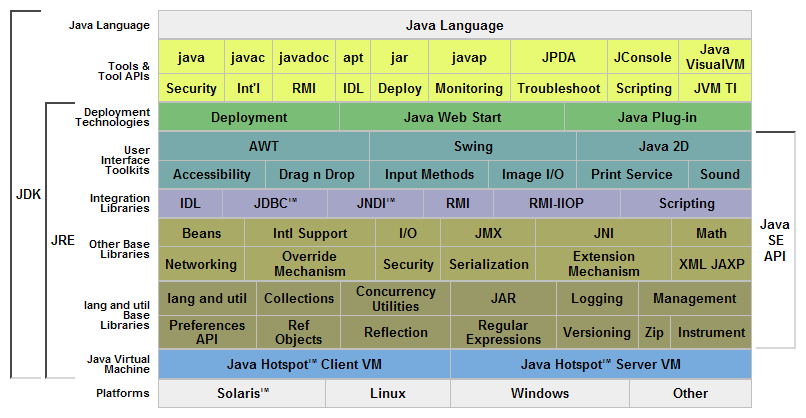
\includegraphics[height=200px, width=320px]{images/JavaPlatform.png}
\end{frame}

\begin{frame}{Езикът Java}
  \transdissolve
  \begin{columns}
    \column{.5\textwidth}
    Column Number 1
    \begin{itemize}
      \item one
      \item two
      \item three
    \end{itemize}
    \column{.5\textwidth}
    Column Number 2
    \begin{itemize}
      \item one
      \item two
      \item three
    \end{itemize}

  \end{columns}
\end{frame}

\section{Groovy}
\subsection{Основни характеристики на Groovy}
\subsection{Groovy в действие}

\begin{frame}{Groovy е...}
  \transdissolve
  \begin{itemize}
  \item Динамичен език за JVM
    \begin{itemize}
      \item Програмите на Groovy директно се компилират до байт код
    \end{itemize}

  \item Вдъхновен от езици като Ruby, Python и Smalltalk
  \item Създаден за да улесни живота на (Java) програмистите
  \item Проект с отворен код, лицензиран под Apache Public License
  \item С граматика директно извлечена от Java 5
    \begin{itemize}
      \item поддържа анотации, generics, изброени типове(enums),
        статични импорти и т.н.
    \end{itemize}

  \end{itemize}
\end{frame}

\begin{frame}{Ключови характеристики}
  \transdissolve
  \begin{itemize}
  \item Напълно обектно-ориентиран
  \item Типизирането не е задължително
  \item Няма нужда да чакате Java 7/8/9:
    \begin{itemize}
      \item Closures - преизползваеми / присвоими блокове код
      \item Атрибути - автоматично генерирани getter/setter методи
    \end{itemize}
  \item Duck typing - типът на обектите се определя от техния
    интерфейс, а не от техния клас
  \item Аритметика базирана на BigDecimal
  \item Улеснена работа с SQL, XML, Swing и т.н.
  \end{itemize}
\end{frame}

\begin{frame}{Java интеграция}
  \transdissolve
  \begin{itemize}
  \item Groovy генерира Java байткод за JVM
    \begin{itemize}
      \item Същите низове, регулярни изрази и т.н.
      \item Същите API
      \item Същия модел на сигурност, същия нишков модел
      \item Същите ОО концепции
      \item Комбинирана компилация
    \end{itemize}
  \end{itemize}
\end{frame}

\begin{frame}{Инсталация}
  \transdissolve
  \begin{itemize}
  \item Идете на http://groovy.codehaus.org
  \item Изтеглете Groovy 1.7
  \item Разархивирайте и установете променливата GROOVY\_HOME
  \item Добавете GROOVY\_HOME/bin в пътя ви
  \item Това е 
  \end{itemize}
\end{frame}

\begin{frame}{Инструменти}
  \transdissolve
  \begin{itemize}
  \item 
  \end{itemize}
\end{frame}


\subsection{Синтаксис на Groovy}
\begin{frame}[fragile]
  \frametitle{Java програма}
  \transdissolve
\begin{lstlisting}
  
\end{lstlisting}
\end{frame}

\begin{frame}[fragile]
  \frametitle{Groovy програма}
  \transdissolve
\begin{lstlisting}
  
\end{lstlisting}
\end{frame}

\begin{frame}{Синтактични конструкции}
  \transdissolve
  \begin{itemize}
  \item Списъци(lists)
    \begin{itemize}
    \item def numbers = [1, 2, 3]      
    \end{itemize}
  \item Асоциативни масиви(maps)
    \begin{itemize}
    \item def map = [BG: "`Bulgaria", DE: "`Germany"]      
    \end{itemize}
  \item Обхват(range)
    \begin{itemize}
      \item def range = 1..1000
    \end{itemize}
  \item Регулярни изрази
    \begin{itemize}
      \item def whitespace = ~/\\s+/
    \end{itemize}

  \end{itemize}
\end{frame}

\begin{frame}{Groovy низове}
  \transdissolve
  \begin{itemize}
  \item GStrings - интерполирани низове
  \item Многоредови низове
  \item Специален синтаксис
  \end{itemize}
\end{frame}

\begin{frame}{Closures}
  \transdissolve
  \begin{itemize}
  \item Преизползваем / присвоим блок код
  \item 
  \end{itemize}
\end{frame}

\begin{frame}{Удобства}
  \transdissolve
  \begin{itemize}
  \item 
  \end{itemize}
\end{frame}

\subsection{Интересни Groovy API}
\begin{frame}{Groovy Dev Kit(GDK)}
  \transdissolve
  \begin{itemize}
  \item Groovy "`декорира" съществуващите JDK API
  \begin{itemize}
    \item Не можем да разширим java.lang.String или java.io.File?
  \end{itemize}

  \end{itemize}
\end{frame}

\begin{frame}{JDBC}
  \transdissolve
  \begin{itemize}
  \item 
  \end{itemize}
\end{frame}

\begin{frame}{XML}
  \transdissolve
  \begin{itemize}
  \item 
  \end{itemize}
\end{frame}

\begin{frame}{Swing}
  \transdissolve
  \begin{itemize}
  \item 
  \end{itemize}
\end{frame}


\section{Scala}
\subsection{Основни характеристики на Scala}
\subsection{Scala в действие}

\begin{frame}{Scala}
  \transdissolve
  \begin{itemize}
  \item 
  \end{itemize}
\end{frame}


\section{Clojure}
\subsection{Основни характеристики на Clojure}
\begin{frame}{Clojure}
  \transdissolve
  \begin{itemize}
  \item 
  \end{itemize}
\end{frame}


\section{Заключение}

\begin{frame}{Заключение}
  \transdissolve
  % Keep the summary *very short*.
  \begin{itemize}
  \item
    Примитивните типове от данни са в основата на \alert{всички} Java приложения.
  \item
    Управляващите конструкции ви позволяват да манипулирате потокът на
    изпълнение на една Java програма.
  \item
    Масивите предоставят начин за групиране на свързани елементи.
  \end{itemize}
  
  % The following outlook is optional.
  \vskip0pt plus.5fill
  \begin{itemize}
  \item
    Следващият път:
    \begin{itemize}
    \item
      Основи на ООП
    \item
      Обекти и класове в Java
    \end{itemize}
  \end{itemize}
\end{frame}


\begin{frame}{Въпроси}
  \transdissolve
  \begin{center}
    \LARGEТук е момента да зададете вашите въпроси! :-)
  \end{center}
\end{frame}


\begin{frame}{Край}
  \transdissolve
  \begin{center}
    \LARGEБлагодаря Ви за вниманието!
  \end{center}
  
\end{frame}


\end{document}


%%% Local Variables: 
%%% mode: latex
%%% TeX-master: t
%%% End: 
